%  Time 01: 
%    Gate 00 h(s0) 
%  Time 02: 
%    Gate 01 cnot(s0,s1) 
%  Time 03: 
%    Gate 02 cnot(q0,s0) 
%    Gate 03 nop(s1) 
%  Time 04: 
%    Gate 04 cnot(q1,s1) 
%  Time 05: 
%    Gate 05 cnot(s0,s1) 
%  Time 06: 
%    Gate 06 h(s0) 
%    Gate 08 nop(s1) 
%  Time 07: 
%    Gate 07 measure(s0) 
%    Gate 09 measure(s1) 
%  Time 08: 
%    Gate 10 cnot(s0,c0) 
%    Gate 11 nop(s1) 
%  Time 09: 
%    Gate 12 cnot(s1,c1) 
%    Gate 13 space(s0) 
%  Time 10: 
%    Gate 14 zero(s0) 
%    Gate 15 zero(s1) 
%  Time 11: 
%    Gate 16 h(s0) 
%  Time 12: 
%    Gate 17 cnot(s0,s1) 
%  Time 13: 
%    Gate 18 cnot(q1,s0) 
%    Gate 19 nop(s1) 
%  Time 14: 
%    Gate 20 cnot(q2,s1) 
%  Time 15: 
%    Gate 21 cnot(s0,s1) 
%  Time 16: 
%    Gate 22 h(s0) 
%    Gate 24 nop(s1) 
%  Time 17: 
%    Gate 23 measure(s0) 
%    Gate 25 measure(s1) 
%  Time 18: 
%    Gate 26 synd(s0,s1,c0,c1) 
%  Time 19: 
%    Gate 27 rop(s0,s1,c0,c1,q0,q1,q2) 

% Qubit circuit matrix:
%% q0: n  , n  , gCxA, n  , n  , n  , n  , n  , n  , n  , n  , n  , n  , n  , n  , n  , n  , n  , gSxA, n   
% q1: n  , n  , n  , gDxB, n  , n  , n  , n  , n  , n  , n  , n  , gMxB, n  , n  , n  , n  , n  , gSxB, n   
% q2: n  , n  , n  , n  , n  , n  , n  , n  , n  , n  , n  , n  , n  , gNxC, n  , n  , n  , n  , gSxC, n   
% s0: gAxD, gBxD, gCxD, n  , gExD, gFxD, gGxD, gHxD, gIxD, gJxD, gKxD, gLxD, gMxD, n  , gOxD, gPxD, gQxD, gRxD, gSxD, N   
% s1: n  , gBxE, gCxE, gDxE, gExE, gFxE, gGxE, gHxE, gIxE, gJxE, n  , gLxE, gMxE, gNxE, gOxE, gPxE, gQxE, gRxE, gSxE, N   
% c0: N  , N  , N  , N  , N  , N  , N  , gHxF, N  , N  , N  , N  , N  , N  , N  , N  , N  , gRxF, gSxF, N   
% c1: N  , N  , N  , N  , N  , N  , N  , N  , gIxG, N  , N  , N  , N  , N  , N  , N  , N  , gRxG, gSxG, N   

\documentclass[11pt]{article}
%
% File:   xyqcirc.tex
% Date:   14-Mar-04
% Author: I. Chuang <ichuang@mit.edu>
%
% Definitions for producing quantum circuits with XYPIC in latex
%
% $Log: xyqcirc.tex,v $
% Revision 1.17  2004/03/25 05:01:23  ike
% discard and slash
%
% Revision 1.16  2004/03/25 04:58:42  ike
% added discard, and variable width dmeter
%
% Revision 1.15  2004/03/24 23:43:33  ike
% \dmeter and \sq
%
% Revision 1.14  2004/03/24 20:29:40  ike
% added \t for swap
%
% Revision 1.13  2004/03/24 17:52:16  ike
% removed \w from \gspace
%
% Revision 1.12  2004/03/24 16:38:34  ike
% added small space before |0> for \z
%
% Revision 1.11  2004/03/24 16:23:11  ike
% added \z
%
% Revision 1.10  2004/03/24 16:19:11  ike
% added multiple qubit operations
%
% Revision 1.9  2004/03/24 03:03:44  ike
% typo
%
% Revision 1.8  2004/03/24 02:50:09  ike
% added qv
%
% Revision 1.7  2004/03/24 00:07:34  ike
% add \m matrix op
%
% Revision 1.6  2004/03/23 23:13:10  ike
% misc
%
% Revision 1.5  2004/03/23 23:12:42  ike
% works now
%
% Revision 1.4  2004/03/23 22:22:34  ike
% ifthen also failes - because xymatrix entries in \save...\restore
%
% Revision 1.3  2004/03/23 21:34:36  ike
% no q/c wire switching
%
% Revision 1.2  2004/03/23 21:25:29  ike
% classical qo quantum wire switching try
%
% Revision 1.1  2004/03/23 21:01:46  ike
% Initial revision
%

%%%%%%%%%%%%%%%%%%%%%%%%%%%%%%%%%%%%%%%%%%%%%%%%%%%%%%%%%%%%%%%%%%%%%%%%%%%%%
% preliminaries

\usepackage{graphicx}

\usepackage[frame,line,arrow,matrix,tips]{xy}	% all that is usually necessary
\CompilePrefix{xygui-}
\makeindex
\pagestyle{empty}

\setlength{\oddsidemargin}{-0.5in}	% 1.25in left margin 
\setlength{\evensidemargin}{-0.5in}	% 1.25in left margin (even pages)

\setlength{\topmargin}{0.0in}		% 1in top margin
\setlength{\textwidth}{6.25in}		% 6.0in text - 1.25in rt margin
\setlength{\textheight}{8.6in}		% Body ht for 1in margins
\addtolength{\topmargin}{-\headheight}	% No header, so compensate
\addtolength{\topmargin}{-\headsep}	% for header height and separation

\begin{document}

\thispagestyle{empty}

%%%%%%%%%%%%%%%%%%%%%%%%%%%%%%%%%%%%%%%%%%%%%%%%%%%%%%%%%%%%%%%%%%%%%%%%%%%%%
% wires

\def\w{\ar@{-}[l]}
\def\W{\ar@{=}[l]}

%%%%%%%%%%%%%%%%%%%%%%%%%%%%%%%%%%%%%%%%%%%%%%%%%%%%%%%%%%%%%%%%%%%%%%%%%%%%%
% labels

% simple label
\def\A#1{\save []="#1" \restore}

%%%%%%%%%%%%%%%%%%%%%%%%%%%%%%%%%%%%%%%%%%%%%%%%%%%%%%%%%%%%%%%%%%%%%%%%%%%%%
% single qubit operations

\def\op#1{*+[F]{\rule[-0.2ex]{0ex}{2.1ex}#1}}	% operator in box
\def\b{*={\bullet}}
\def\o{*={\oplus}}
\def\t{*={\times}}				% for swap gate
\def\sq{*=<6pt,6pt>[F]{}}			% square, for controlled-phase
\def\m#1{\left[\matrix{#1}\right]}		% matrix shortcut
\def\z{*+[]{\rule[-0.2ex]{0ex}{2.1ex}~|0\>}}	% re-init to |0>
\def\discard{*[]{\rule[-0.2ex]{0.75pt}{2.1ex}~}}	% vertical ``|''
\def\slash{*={/}}				% slash for wire bundles

%%%%%%%%%%%%%%%%%%%%%%%%%%%%%%%%%%%%%%%%%%%%%%%%%%%%%%%%%%%%%%%%%%%%%%%%%%%%%
% nop's

\def\N{*-{}\W}
\def\n{*-{}\w}

%%%%%%%%%%%%%%%%%%%%%%%%%%%%%%%%%%%%%%%%%%%%%%%%%%%%%%%%%%%%%%%%%%%%%%%%%%%%%
% misc definitions

\def\>{\rangle}
\def\<{\langle}
\def\ua{\uparrow}

% measurement box
\def\meter{*+[]{\put(-3,0){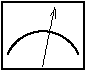
\includegraphics[scale=.5]{meter}}~~~~}%
		\ar@{-}[l]}

%%%%%%%%%%%%%%%%%%%%%%%%%%%%%%%%%%%%%%%%%%%%%%%%%%%%%%%%%%%%%%%%%%%%%%%%%%%%%
% qubit names (and also revert to qubit wires, vs, cbit wires)

\def\q#1{*+{\rule[-0.2ex]{0ex}{2.1ex}|#1\>}}
\def\qv#1#2{*+{\rule[-0.2ex]{0ex}{2.1ex}|#1\>=|#2\>}}
	
%%%%%%%%%%%%%%%%%%%%%%%%%%%%%%%%%%%%%%%%%%%%%%%%%%%%%%%%%%%%%%%%%%%%%%%%%%%%%
% multiple qubit gates

% utulity text box for figuring out width of things
\newbox{\sbox}

% empty space of width determined by the text argument
\def\gspace#1{*+{\rule[-0.2ex]{0ex}{2.1ex}%
	\setbox\sbox=\hbox{$#1$}%
	\hspace*{\wd\sbox}}}
	
% n-qubit operation #1=box label, #2=number of qubits (eg d=2 qubits, ddd=4)
\def\gnqubit#1#2{\gspace{#1}
		 \save [].[#2]!C="qq"*[F]\frm{}\restore
		 \save "qq"*[]{#1} \restore}

% two-qubit operation
\def\gtwo#1{\gnqubit{#1}{d}}

% two-qubit operation
\def\gthree#1{\gnqubit{#1}{dd}}

%%%%%%%%%%%%%%%%%%%%%%%%%%%%%%%%%%%%%%%%%%%%%%%%%%%%%%%%%%%%%%%%%%%%%%%%%%%%%
% ``D'' style measurement gate a-la-cleve, at Michael Nielsen's request

\def\dmeterwide#1#2{*{\xy <0pt,-8pt>;<0pt,8pt> **@{-};
		    <0pt,-8pt>;<#2,-8pt> **@{-} ;
		    <0pt, 8pt>;<#2, 8pt> **@{-} ;
		    <#2,0pt>-<5pt,0pt>*{#1} ;
		    <#2,0pt>*\cir<8pt>{r_l}\endxy}}

\def\dmeter#1{\dmeterwide{#1}{12pt}}

%%%%%%%%%%%%%%%%%%%%%%%%%%%%%%%%%%%%%%%%%%%%%%%%%%%%%%%%%%%%%%%%%%%%%%%%%%%%%


% definitions for the circuit elements 
\def\gAxD{\op{H}\w\A{gAxD}}
\def\gBxD{\b\w\A{gBxD}}
\def\gBxE{\o\w\A{gBxE}}
\def\gCxA{\b\w\A{gCxA}}
\def\gCxD{\o\w\A{gCxD}}
\def\gCxE{*-{}\w\A{gCxE}}
\def\gDxB{\b\w\A{gDxB}}
\def\gDxE{\o\w\A{gDxE}}
\def\gExD{\b\w\A{gExD}}
\def\gExE{\o\w\A{gExE}}
\def\gFxD{\op{H}\w\A{gFxD}}
\def\gGxD{\meter\w\A{gGxD}}
\def\gFxE{*-{}\w\A{gFxE}}
\def\gGxE{\meter\w\A{gGxE}}
\def\gHxD{\b\W\A{gHxD}}
\def\gHxF{\o\W\A{gHxF}}
\def\gHxE{*-{}\W\A{gHxE}}
\def\gIxE{\b\W\A{gIxE}}
\def\gIxG{\o\W\A{gIxG}}
\def\gIxD{\A{gIxD}}
\def\gJxD{\z\A{gJxD}}
\def\gJxE{\z\A{gJxE}}
\def\gKxD{\op{H}\w\A{gKxD}}
\def\gLxD{\b\w\A{gLxD}}
\def\gLxE{\o\w\A{gLxE}}
\def\gMxB{\b\w\A{gMxB}}
\def\gMxD{\o\w\A{gMxD}}
\def\gMxE{*-{}\w\A{gMxE}}
\def\gNxC{\b\w\A{gNxC}}
\def\gNxE{\o\w\A{gNxE}}
\def\gOxD{\b\w\A{gOxD}}
\def\gOxE{\o\w\A{gOxE}}
\def\gPxD{\op{H}\w\A{gPxD}}
\def\gQxD{\meter\w\A{gQxD}}
\def\gPxE{*-{}\w\A{gPxE}}
\def\gQxE{\meter\w\A{gQxE}}
\def\gRxD{\gnqubit{\txt{Process\\Syndrome}}{ddd}\W\A{gRxD}}
\def\gRxE{\gspace{\txt{Process\\Syndrome}}\W\A{gRxE}}
\def\gRxF{\gspace{\txt{Process\\Syndrome}}\W\A{gRxF}}
\def\gRxG{\gspace{\txt{Process\\Syndrome}}\W\A{gRxG}}
\def\gSxA{\gnqubit{{\cal R}}{dd}\w\A{gSxA}}
\def\gSxB{\gspace{{\cal R}}\w\A{gSxB}}
\def\gSxC{\gspace{{\cal R}}\w\A{gSxC}}
\def\gSxD{\b\W\A{gSxD}}
\def\gSxE{\b\W\A{gSxE}}
\def\gSxF{\b\W\A{gSxF}}
\def\gSxG{\b\W\A{gSxG}}

% definitions for bit labels and initial states 
\def\bA{ \q{q_{0}}}
\def\bB{ \q{q_{1}}}
\def\bC{ \q{q_{2}}}
\def\bD{\qv{s_{0}}{0}}
\def\bE{\qv{s_{1}}{0}}
\def\bF{   {c_{0} = 0}}
\def\bG{   {c_{1} = 0}}

% The quantum circuit as an xymatrix 
\xymatrix@R=5pt@C=10pt{ 
    \bA & \n   &\n   &\gCxA &\n   &\n   &\n   &\n   &\n   &\n   &\n   &\n   &\n   &\n   &\n   &\n   &\n   &\n   &\n   &\gSxA &\n  
\\  \bB & \n   &\n   &\n   &\gDxB &\n   &\n   &\n   &\n   &\n   &\n   &\n   &\n   &\gMxB &\n   &\n   &\n   &\n   &\n   &\gSxB &\n  
\\  \bC & \n   &\n   &\n   &\n   &\n   &\n   &\n   &\n   &\n   &\n   &\n   &\n   &\n   &\gNxC &\n   &\n   &\n   &\n   &\gSxC &\n  
\\  \bD & \gAxD &\gBxD &\gCxD &\n   &\gExD &\gFxD &\gGxD &\gHxD &\gIxD &\gJxD &\gKxD &\gLxD &\gMxD &\n   &\gOxD &\gPxD &\gQxD &\gRxD &\gSxD &\N  
\\  \bE & \n   &\gBxE &\gCxE &\gDxE &\gExE &\gFxE &\gGxE &\gHxE &\gIxE &\gJxE &\n   &\gLxE &\gMxE &\gNxE &\gOxE &\gPxE &\gQxE &\gRxE &\gSxE &\N  
\\  \bF & \N   &\N   &\N   &\N   &\N   &\N   &\N   &\gHxF &\N   &\N   &\N   &\N   &\N   &\N   &\N   &\N   &\N   &\gRxF &\gSxF &\N  
\\  \bG & \N   &\N   &\N   &\N   &\N   &\N   &\N   &\N   &\gIxG &\N   &\N   &\N   &\N   &\N   &\N   &\N   &\N   &\gRxG &\gSxG &\N  
% 
% Vertical lines and other post-xymatrix latex % 
\ar@{-}"gBxE";"gBxD"\ar@{-}"gCxD";"gCxA"\ar@{-}"gDxE";"gDxB"\ar@{-}"gExE";"gExD"\ar@{=}"gHxF";"gHxD"\ar@{=}"gIxG";"gIxE"\ar@{-}"gLxE";"gLxD"\ar@{-}"gMxD";"gMxB"\ar@{-}"gNxE";"gNxC"\ar@{-}"gOxE";"gOxD"\ar@{=}"gSxC";"gSxD"\ar@{=}"gSxC";"gSxE"\ar@{=}"gSxC";"gSxF"\ar@{=}"gSxC";"gSxG"}
 
\end{document}